\documentclass[a4paper]{article}
\usepackage{ctex}
\usepackage{geometry}
\usepackage{amsmath}
\usepackage{ulem}
\usepackage{graphicx}
\usepackage{siunitx}
\usepackage{enumitem}
\usepackage{multirow}
\usepackage{adjustbox}
\usepackage[hidelinks]{hyperref}
\usepackage{tabularx}
\usepackage{array}
\usepackage{float}
\newcolumntype{Y}{>{\centering\arraybackslash}X}

\geometry{left=2.5cm, right=2.5cm, top=2.5cm, bottom=2.5cm}
\zihao{-4}

\begin{document}

\noindent\textbf{班级：24级整合科学班} \hspace{1cm} \textbf{学号：2400017802} \hspace{1cm} \textbf{姓名：冯翊展} \hspace{1cm} \textbf{评分：}\\
\textbf{同组学生：胡家豪、刘天乐、汪泽睿、张城滔} \\
\textbf{实验名称：光栅衍射观察与光盘刻槽密度测算}   \hfill \textbf{实验日期：2025年4月21日} 

\hrule
\vspace{3mm}

\begin{enumerate}[label=\chinese*.,left=0pt]
    \item 实验目的
    \\
    观察白光与单色光源透过不同线数光栅的分光情况；将CD与DVD光盘视作反射光栅，测算其刻槽密度。
   
    \item 基本原理
    \begin{enumerate}[label=\arabic*.,left=0pt]
        \item 光栅分光原理
        \\
        由大量等宽等间距的平行狭缝构成的光学器件称为光栅，其工作原理是夫琅禾费多缝衍射。当单色光垂直照射到光栅上时，不同方向上的出射光会出现干涉增强，干涉的极大位置满足下面的光栅方程：
        $$d \sin \theta = m \lambda$$
        其中 $d$ 是光栅常数，$m$ 是衍射级数（$0,\pm1,\pm2,...$），$\theta$ 是第 $m$ 级衍射角，$\lambda$ 是入射光的波长。衍射角 $\theta$ 可以通过光栅与光屏的距离 $L$ 和 中心（零级）到 $m$ 级衍射光斑的距离 $x$计算：
        $$\tan \theta = \frac{x}{L}$$

        \item CD与DVD光盘
        \\
        CD与DVD通过反面的同心圆形刻槽来记录数据，可以近似认为其为均匀反射光栅，其中每一圈凹槽或反射区相当于一条栅线，因此光栅常数 $d$ 就等于数据轨道间距，即刻槽密度 $N$ 的倒数。
    \end{enumerate}
   
    
        

    
    \item 仪器与试剂
    \\
    强光手电筒、红色（\qty{650}{\nm}）激光笔、绿色（\qty{532}{\nm}）激光笔、500/1000线光栅、CD光盘、DVD光盘、卷尺

    \item 实验步骤
    \begin{enumerate}[label=\arabic*.,left=0pt]
        \item 取500线和1000线光栅各一个，使用强光手电筒照射，观察分光情况并记录。
        \item 改用红色与绿色激光笔，重复实验。
        \item 利用CD光盘作为反射光栅，重复实验，记录数据，测算其刻槽密度。
        \item 利用DVD光盘作为反射光栅，重复实验，记录数据，测算其刻槽密度。
    \end{enumerate}
    
    \item 实验结果与分析
    \begin{enumerate}[label=\arabic*.,left=0pt]
        \item 光栅分光情况观察
        \\ 使用强光手电筒（白光）、红光激光笔、绿光激光笔照射500与1000线的光栅，观察到投射光斑如图：
        \begin{figure}[H]
            \centering
            \begin{minipage}{0.395\textwidth}
                \centering
                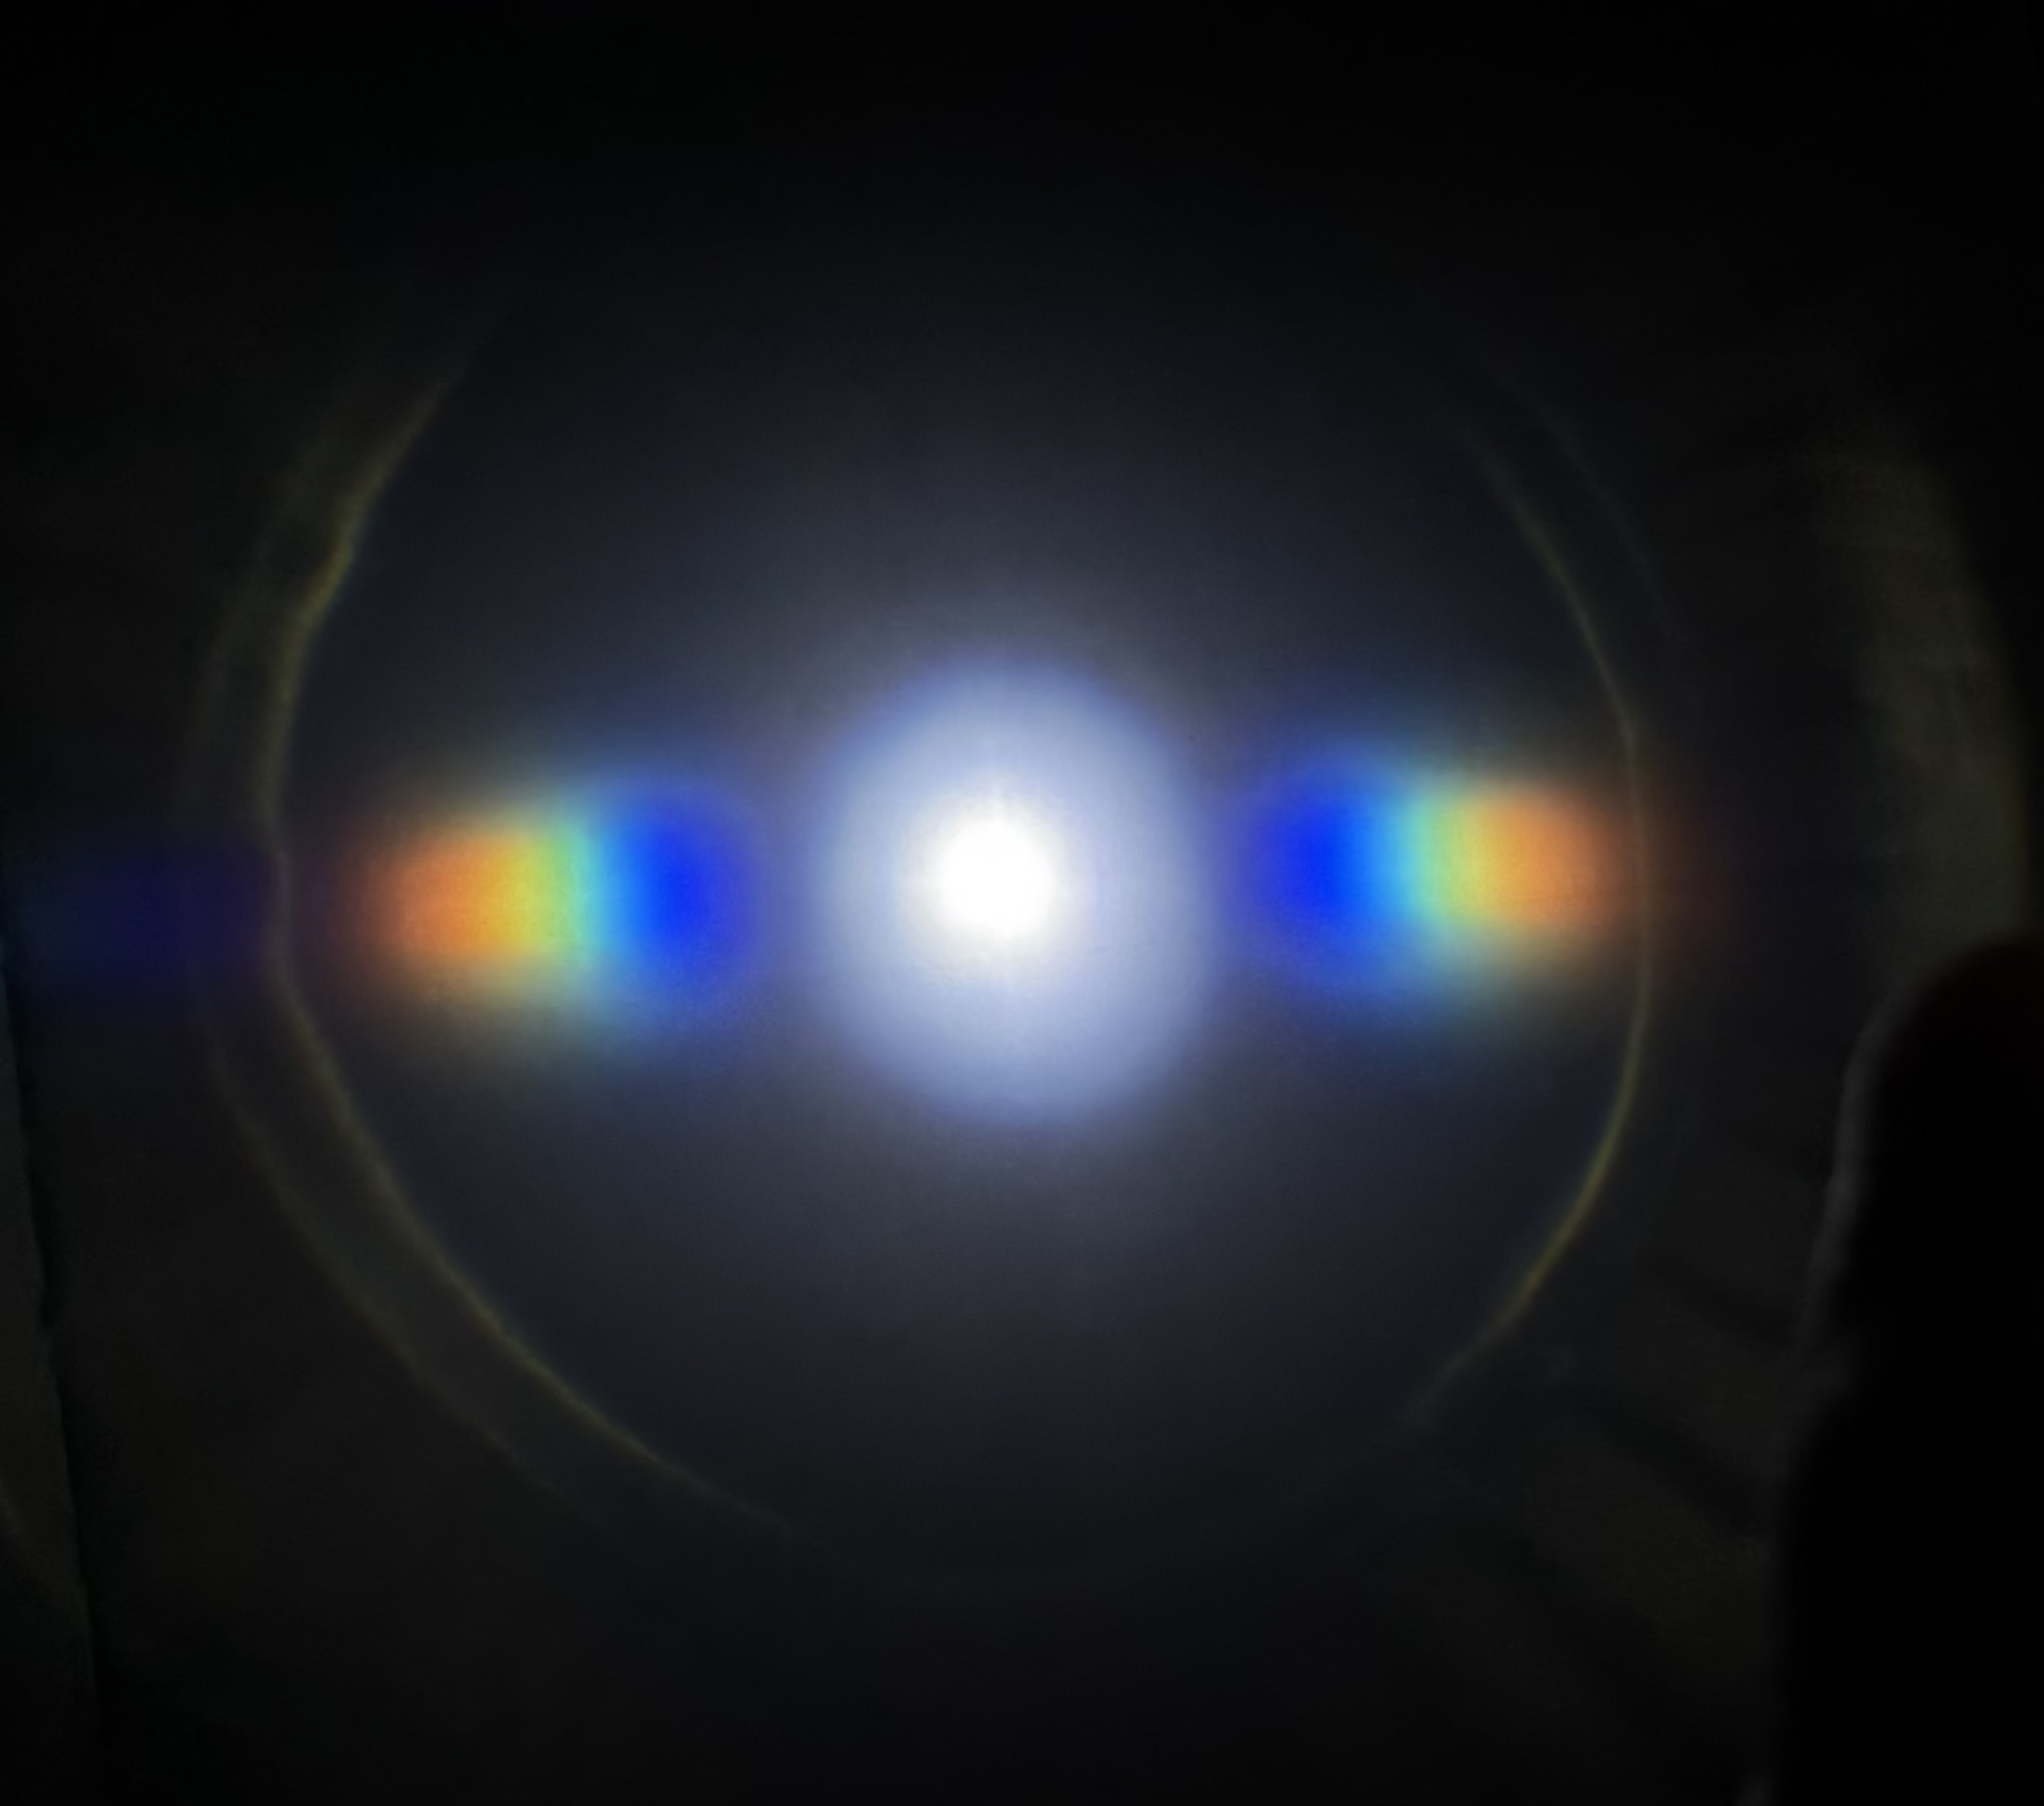
\includegraphics[width=\textwidth]{500W.JPG}
            \end{minipage}
            \begin{minipage}{0.47\textwidth}
                \centering
                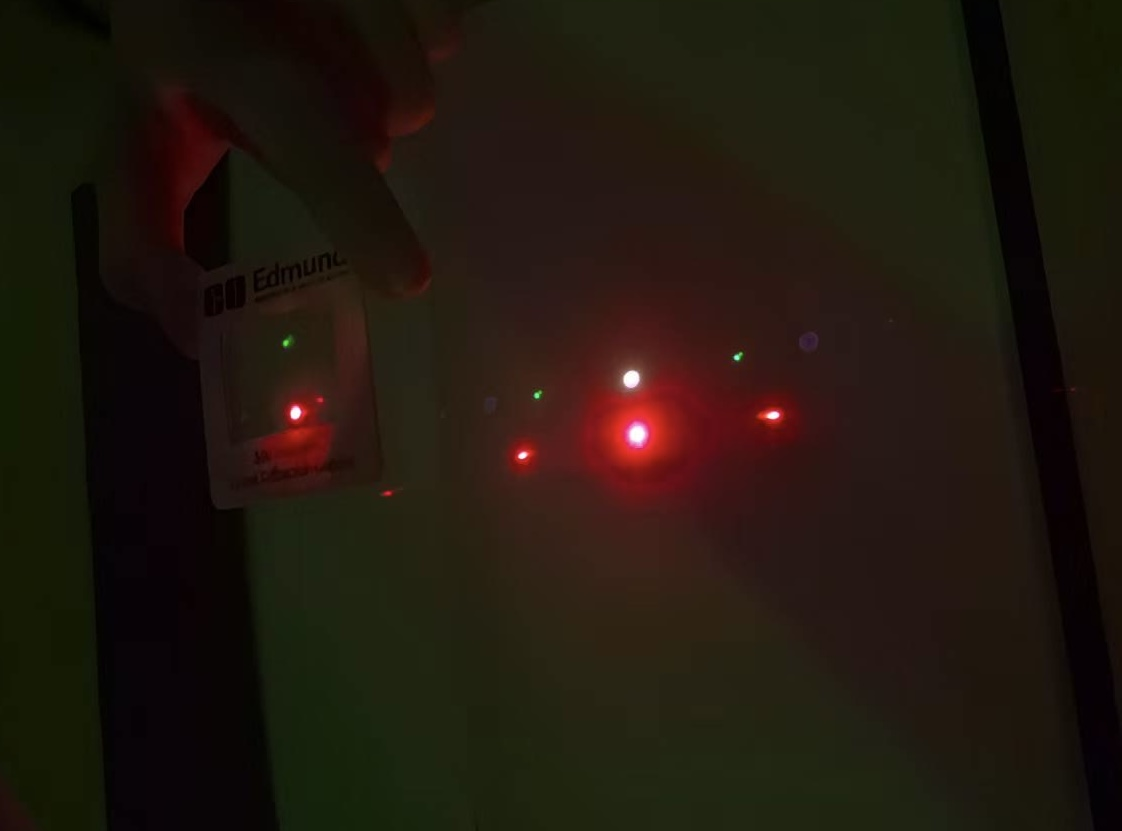
\includegraphics[width=\textwidth]{500RG.jpg}
            \end{minipage}
            \caption{500线光栅分光}
        \end{figure}

        \begin{figure}[H]
            \centering
            \begin{minipage}{0.45\textwidth}
                \centering
                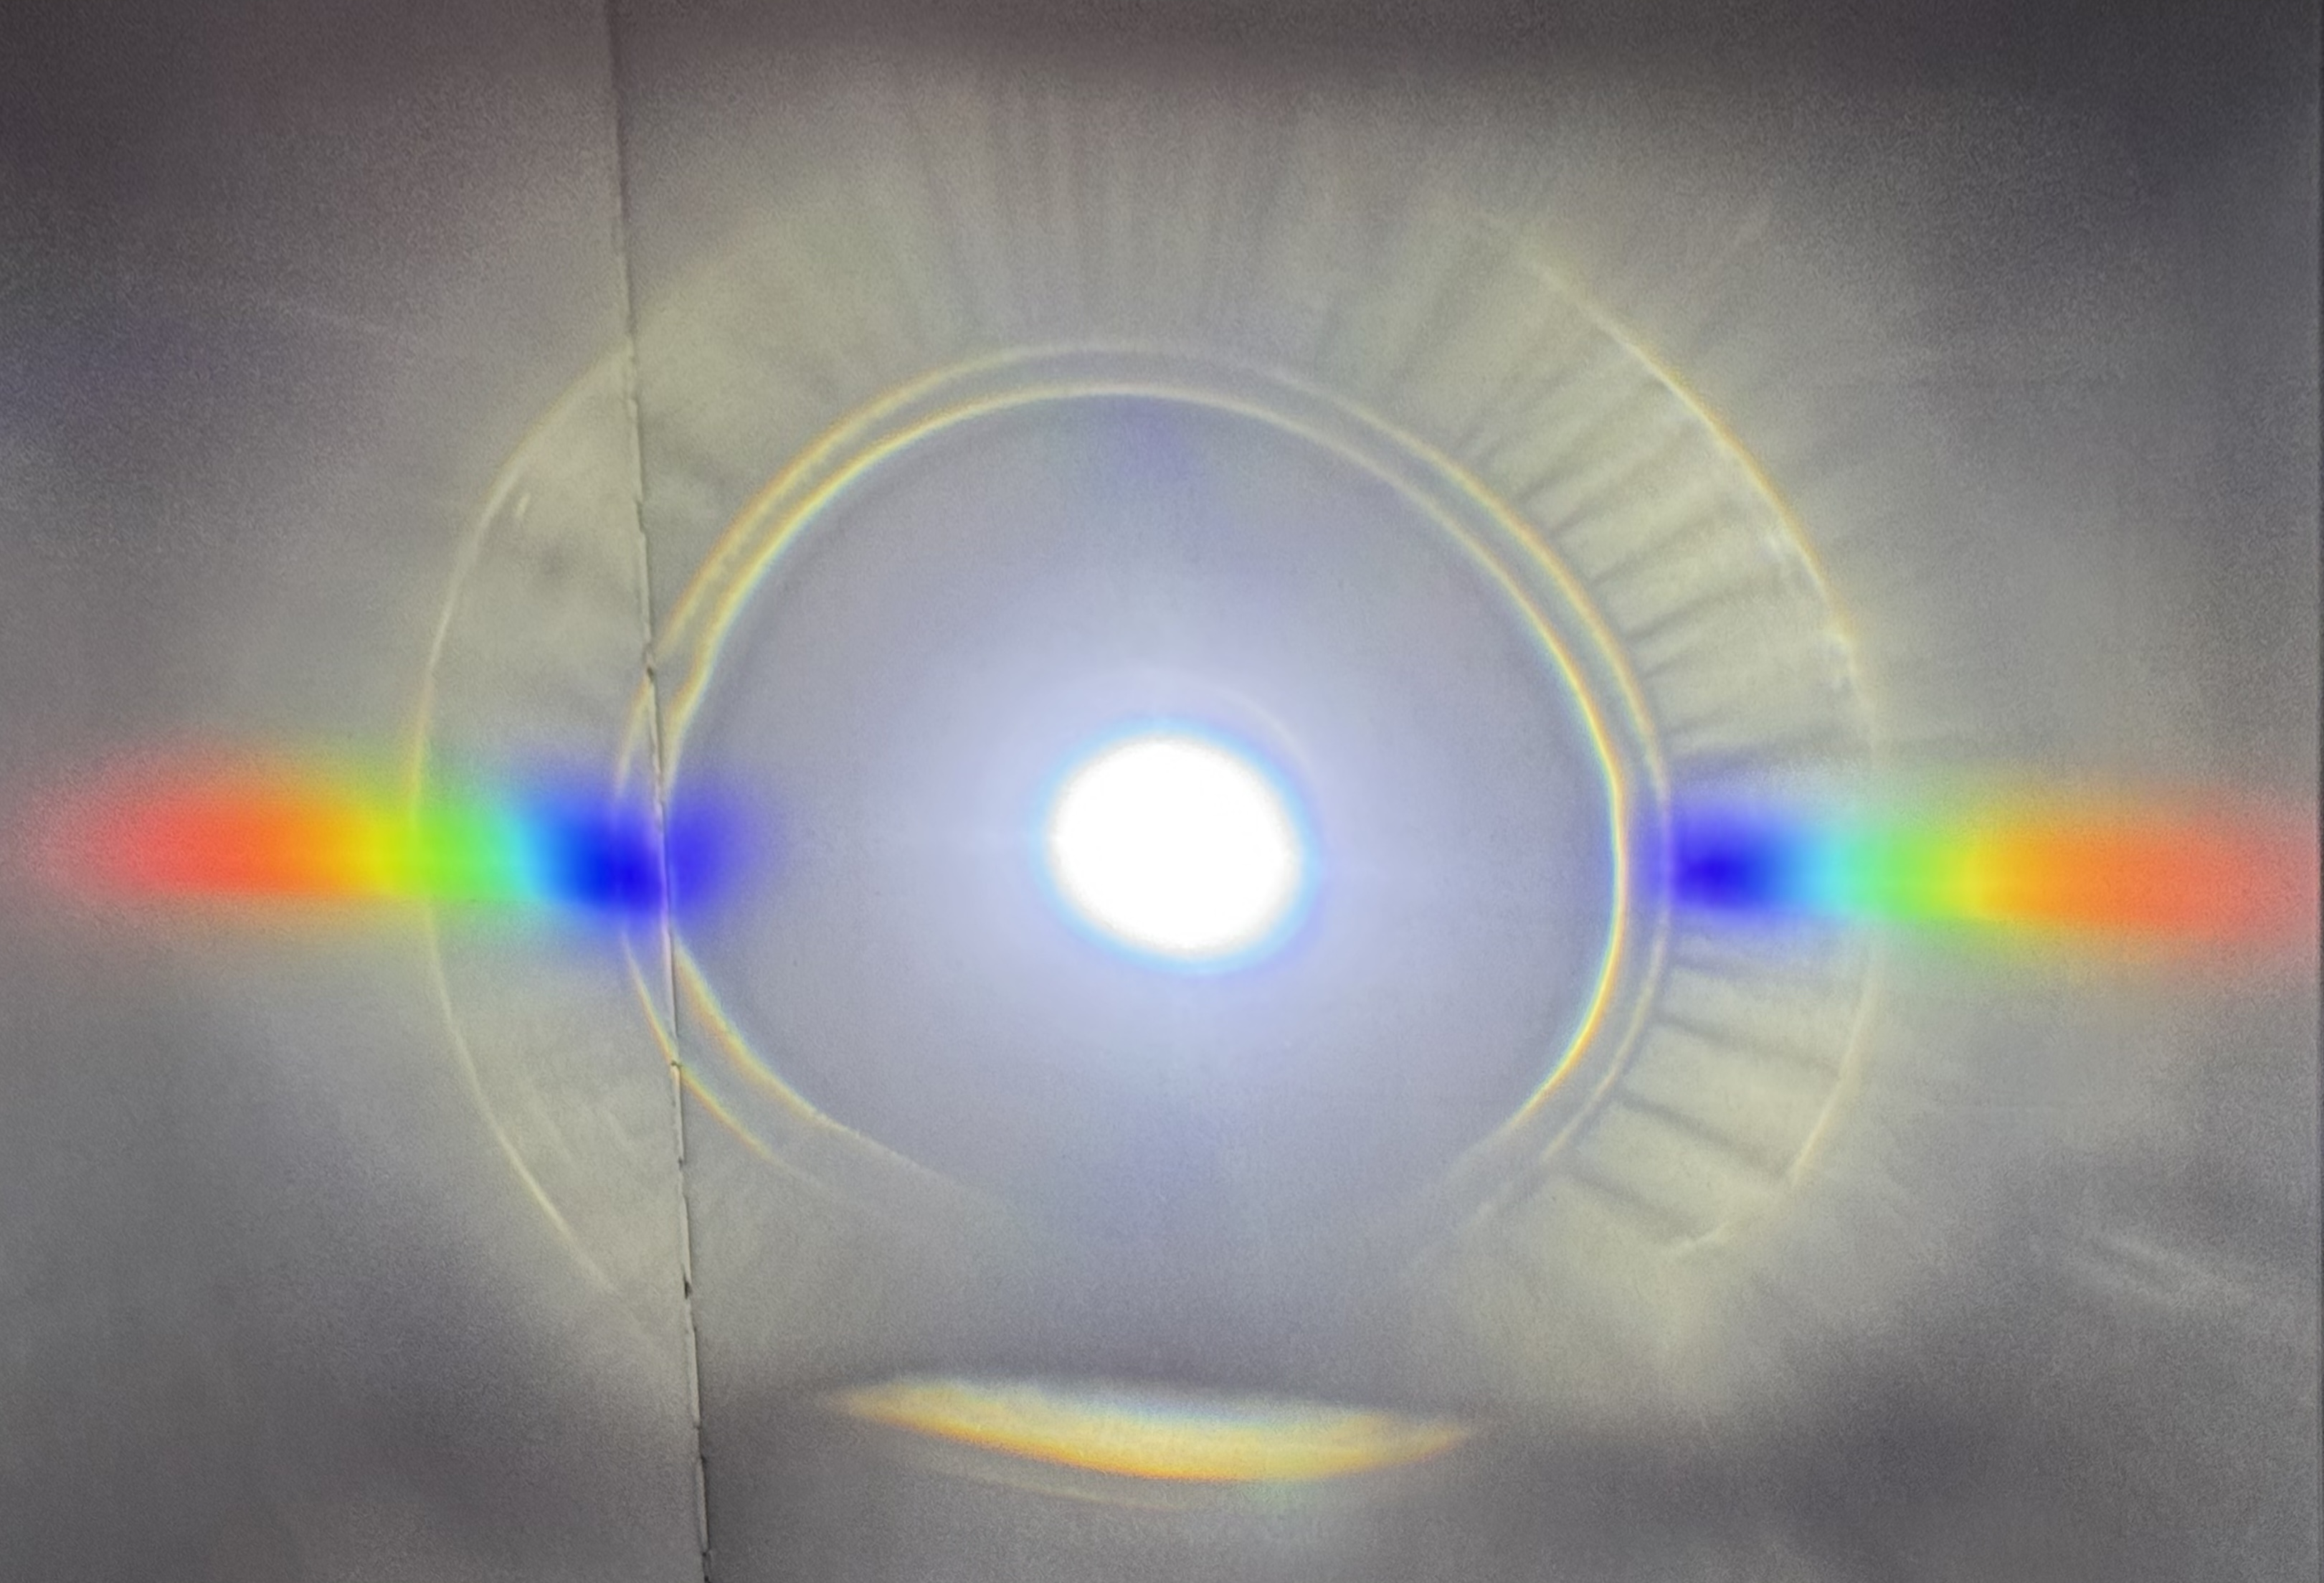
\includegraphics[width=\textwidth]{1000W.jpg}
            \end{minipage}
            \begin{minipage}{0.47\textwidth}
                \centering
                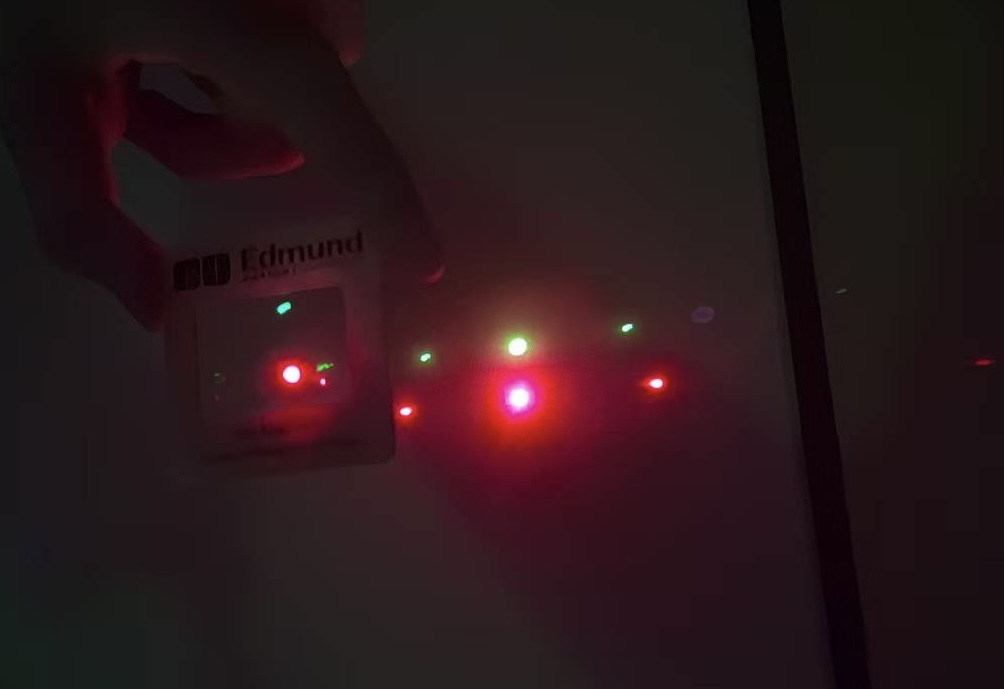
\includegraphics[width=\textwidth]{1000RG.jpg}
            \end{minipage}
            \caption{1000线光栅分光}
        \end{figure}
        从图中可以看出，白光被分光为中心白色亮斑、两边按波长分光形成内紫外红的衍射图案，这符合衍射公式中波长越短，衍射角越小，对应的光斑到衍射中心的距离也更短的规律；对于单色光源，则呈现出有规律的衍射斑点，对应光栅干涉的极大位置；1000线的光栅分光产生的光斑间距更远，符合衍射公式中光栅常数越小，衍射角越大的规律。
        
        \item 光盘刻槽密度计算
        \\
        将CD光盘平行架在离桌面一定高度的位置，使用红色和绿色激光笔垂直向上发射激光，以桌面作为光屏记录衍射条纹的位置，测量条纹与衍射中心的位置。更换CD为DVD重复实验，最终得到以下结果：
        \begin{table}[H]
            \caption{衍射条纹测量数据与计算结果}
            \label{tab:data-2}
            \centering
            \scalebox{1}{ 
            \setlength{\tabcolsep}{6pt}
            \renewcommand{\arraystretch}{1.2} 
            \begin{tabular}{cccccccc}
            光栅类型 & 光源 & $L/\qty{}{\mm}$ & $m$ & $x/\qty{}{\mm}$ & $\theta$ & $d/\qty{}{\um}$ & $N/\qty{}{\per \mm}$  \\ 
            CD & 红（\qty{650}{\nm}）& 170 & 1 & 85.0 & \qty{26.6}{\degree} & 1.45 & 688 \\ 
            CD & 红（\qty{650}{\nm}）& 170 & 2 & 310  & \qty{61.3}{\degree} & 1.48 & 674 \\
            CD & 绿（\qty{532}{\nm}）& 170 & 1 & 60.0 & \qty{19.4}{\degree} & 1.60 & 626 \\
            CD & 绿（\qty{532}{\nm}）& 170 & 2 & 145  & \qty{40.5}{\degree} & 1.64 & 610 \\
            DVD & 红（\qty{650}{\nm}）& 170 & 1 & 328  & \qty{62.6}{\degree} & 0.732 & 1365 \\
            DVD & 绿（\qty{532}{\nm}）& 170 & 1 & 180  & \qty{46.6}{\degree} & 0.732 & 1367 \\
            \end{tabular}
            }
        \end{table}
        查阅标准CD和DVD参数可知，$N_\text{CD} = \qty{625}{\per \mm}$，$N_\text{DVD}=\qty{1351}{\per \mm}$。

        \item 误差分析
        \\
        实验的主要误差来源是对衍射条纹距离的测量。实验使用的激光笔并非理想激光源，而是具有 $\pm\qty{10}{\nm}$ 的波长范围，这使得实验观察到的衍射光斑是一个椭圆形，且越远离衍射中心其畸变程度越高，难以确定中心点位置，因此测量光斑到衍射中心距离时有一定误差。一方面，绿光相比红光波长更短，衍射条纹更加集中，因此测量时误差更小，因此使用绿光测得刻槽密度跟接近理论值；另一方面，由于DVD刻槽密度更高，对应的衍射条纹相比CD更加稀疏，降低了测量的相对误差，使得使用红光和绿光测量时，DVD的刻槽密度都更加接近理论值。
        
    \end{enumerate}
    



\end{enumerate}
\end{document}